\chapter{Analyse du parcours universitaire des bacheliers (UCAD)}

\section{Introduction}

Ce chapitre s'intéresse à la trajectoire des bacheliers, une fois admis à l'université, en particulier à l'UCAD. 
L’objectif est d’évaluer l’impact des différentes réformes du baccalauréat sur l’orientation et la réussite universitaire des étudiants issus des séries concernées.

Dans un premier temps, nous analyserons l’évolution des effectifs inscrits à l’UCAD selon les séries de baccalauréat impactées par les réformes.
Nous observerons ensuite les établissements et départements universitaires où ces bacheliers sont le plus souvent orientés, afin d’identifier les filières de destination privilégiées selon la série d’origine.

Enfin, une analyse de type \textbf{suivi de cohorte} permettra d’évaluer la progression et les performances académiques de ces étudiants dans le temps (réussite, redoublement, abandon), afin de mieux comprendre les effets des réformes sur la réussite universitaire.

\section{Évolution des inscriptions à l'UCAD}

\newpage
\subsection{Les inscrits des série STEG et G}

\begin{figure}[ht]
\centering
\caption{Évolution des inscriptions à l'UCAD pour les séries STEG et G}
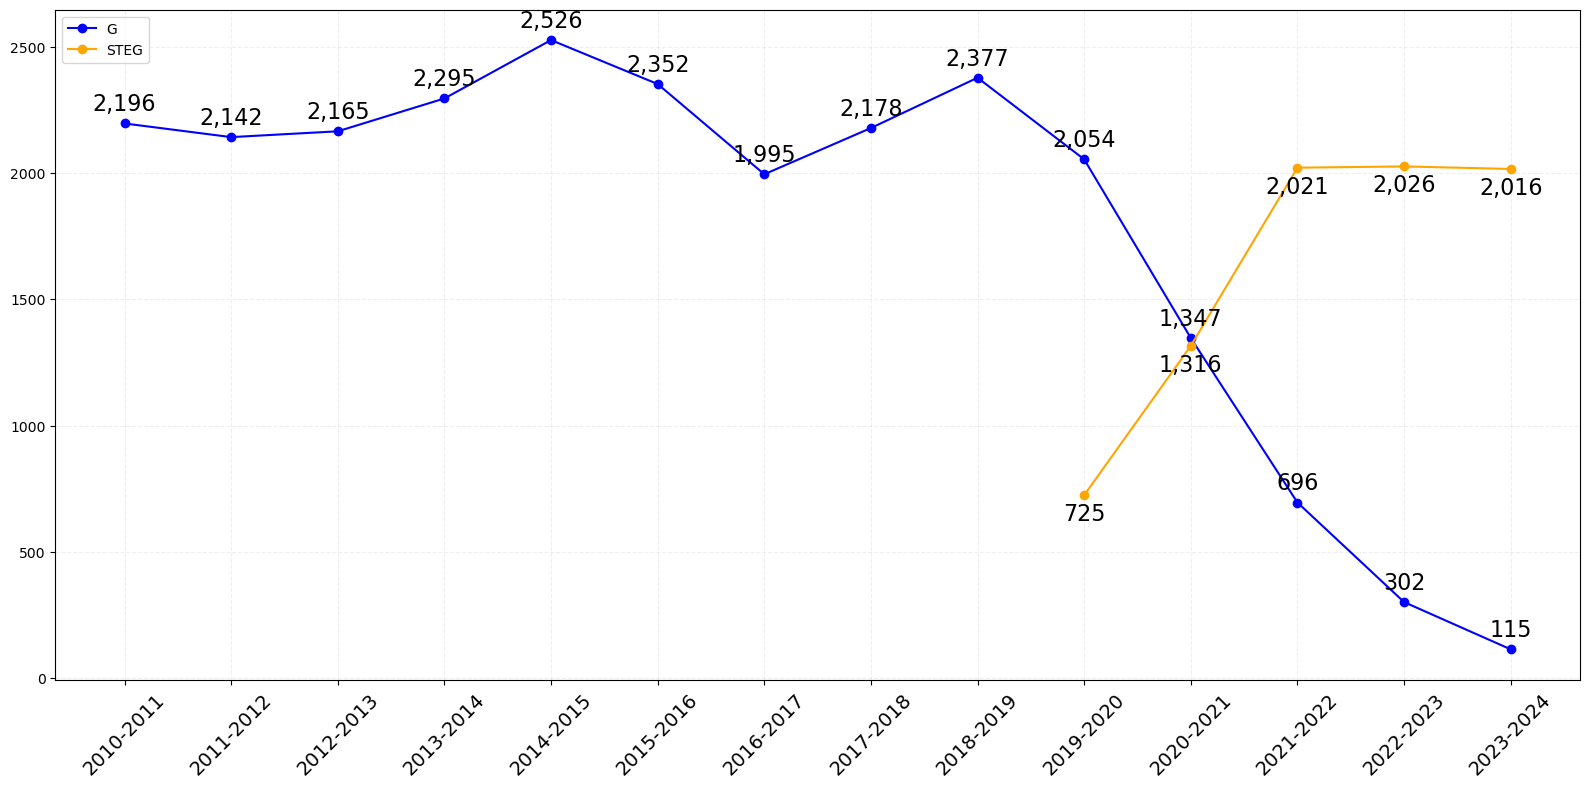
\includegraphics[width=1\textwidth]{figure/Inscrits_ucad_STEG.png}
\label{fig:inscrits_ucad_steg}
\end{figure}

La figure (Figure~\ref{fig:inscrits_ucad_steg}) illustre l'évolution des inscriptions à l'Université Cheikh Anta Diop (UCAD) pour les bacheliers issus des séries G et STEG, sur la période 2010-2011 à 2023-2024.

Jusqu'à l'année universitaire 2018-2019, seule la série G est représentée à l'UCAD, avec un nombre d'inscrits fluctuant autour de 2 000 à 2 500. Un pic est observé en 2014-2015 avec 2 526 inscrits. 
À partir de 2019-2020, la série STEG fait son apparition, avec 725 inscrits, marquant le début de la transition. Simultanément, les effectifs de la série G commencent à décliner fortement, passant de 2 054 en 2019-2020 à seulement 115 en 2023-2024. 
Ce déclin correspond à la suppression progressive de la série G au profit de la série STEG dans le système du baccalauréat.

Le croisement des courbes est particulièrement visible en 2020-2021, où le nombre d'inscrits en STEG (1 347) dépasse celui de la série G (1 316). 
Cette tendance se confirme les années suivantes, la série STEG affichant des effectifs croissants (2 021 en 2021-2022, 2 026 en 2022-2023, et 2 016 en 2023-2024), tandis que la série G continue sa chute. 
La série STEG maintient ainsi un volume d'inscriptions à l'UCAD comparable à celui que la série G connaissait avant sa suppression, démontrant une transition quantitativement réussie au niveau de l'entrée à l'université. 
Ce transfert des effectifs de la série G vers la série STEG à l'UCAD est un indicateur de l'efficacité de la réforme du baccalauréat dans l'orientation des étudiants vers la nouvelle filière.

\newpage
\subsection{Les inscrits des séries Arables et Franco-Arabes}

\subsubsection{Série LA et LAR}

\begin{figure}[ht]
\centering
\caption{Évolution des inscriptions à l'UCAD pour les séries LA et LAR}
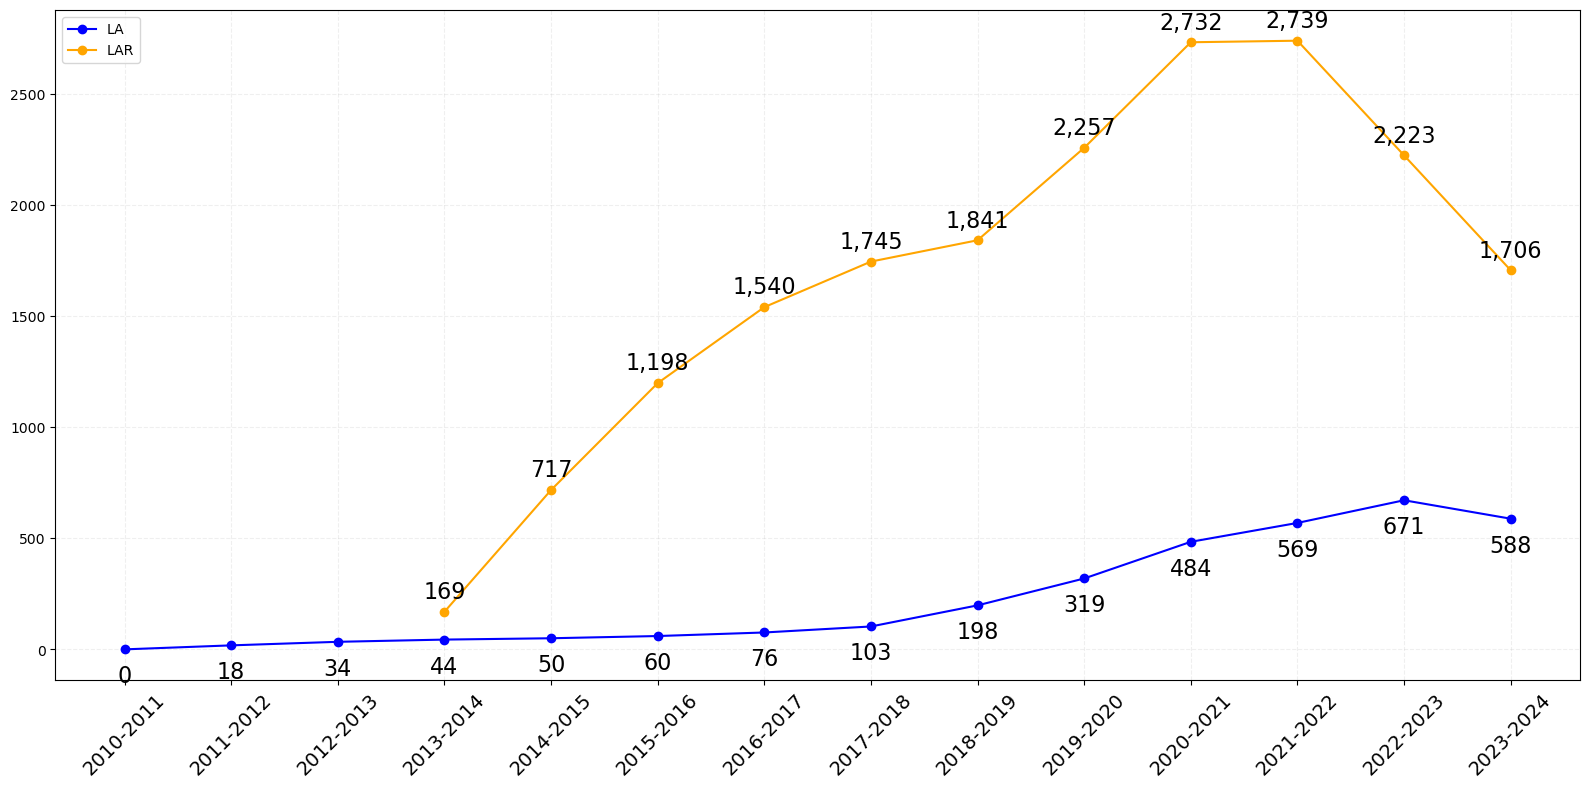
\includegraphics[width=1\textwidth]{figure/Inscrits_ucad_LA_LAR.png}
\label{fig:inscrits_ucad_la_lar}
\end{figure}

La figure (Figure~\ref{fig:inscrits_ucad_la_lar}) présente l'évolution des inscriptions à l'UCAD pour les bacheliers issus des séries Littératures Arabes (LA) et Littératures et Civilisations Arabes (L-AR) de 2010-2011 à 2023-2024.

La série LA, bien que présente depuis 2010-2011, a enregistré un nombre très faible d'inscrits à l'UCAD jusqu'en 2013-2014, oscillant entre 0 et 44. 
À partir de 2014-2015, le nombre d'inscrits en LA connaît une croissance progressive, passant de 50 à 671 en 2022-2023, avant de redescendre légèrement à 588 en 2023-2024.

La série L-AR, introduite à l'UCAD à partir de 2013-2014, a connu une croissance beaucoup plus rapide et significative. Elle débute avec 169 inscrits en 2013-2014 et grimpe rapidement pour atteindre un pic de 2 739 inscrits en 2021-2022. 
Bien qu'une légère diminution soit observée les années suivantes, avec 2 223 inscrits en 2022-2023 et 1 706 en 2023-2024, la série L-AR maintient un volume d'inscriptions considérablement plus élevé que la série LA. 
Ce phénomène s'aligne avec l'observation d'un transfert progressif des effectifs vers la série L-AR au niveau du baccalauréat lui-même, la série L-AR ayant été mise en place pour mieux encadrer et répondre à la demande sociale des filières arabes et franco-arabes. 

% En conclusion, la série L-AR a réussi à s'imposer comme la filière majeure pour les étudiants en études arabes à l'UCAD, absorbant une grande partie des effectifs et démontrant l'impact des réformes du baccalauréat sur l'orientation universitaire.

\newpage
\subsubsection{Série S2A et S1A}

\begin{figure}[ht]
\centering
\caption{Évolution des inscriptions à l'UCAD pour les séries S2A et S1A}
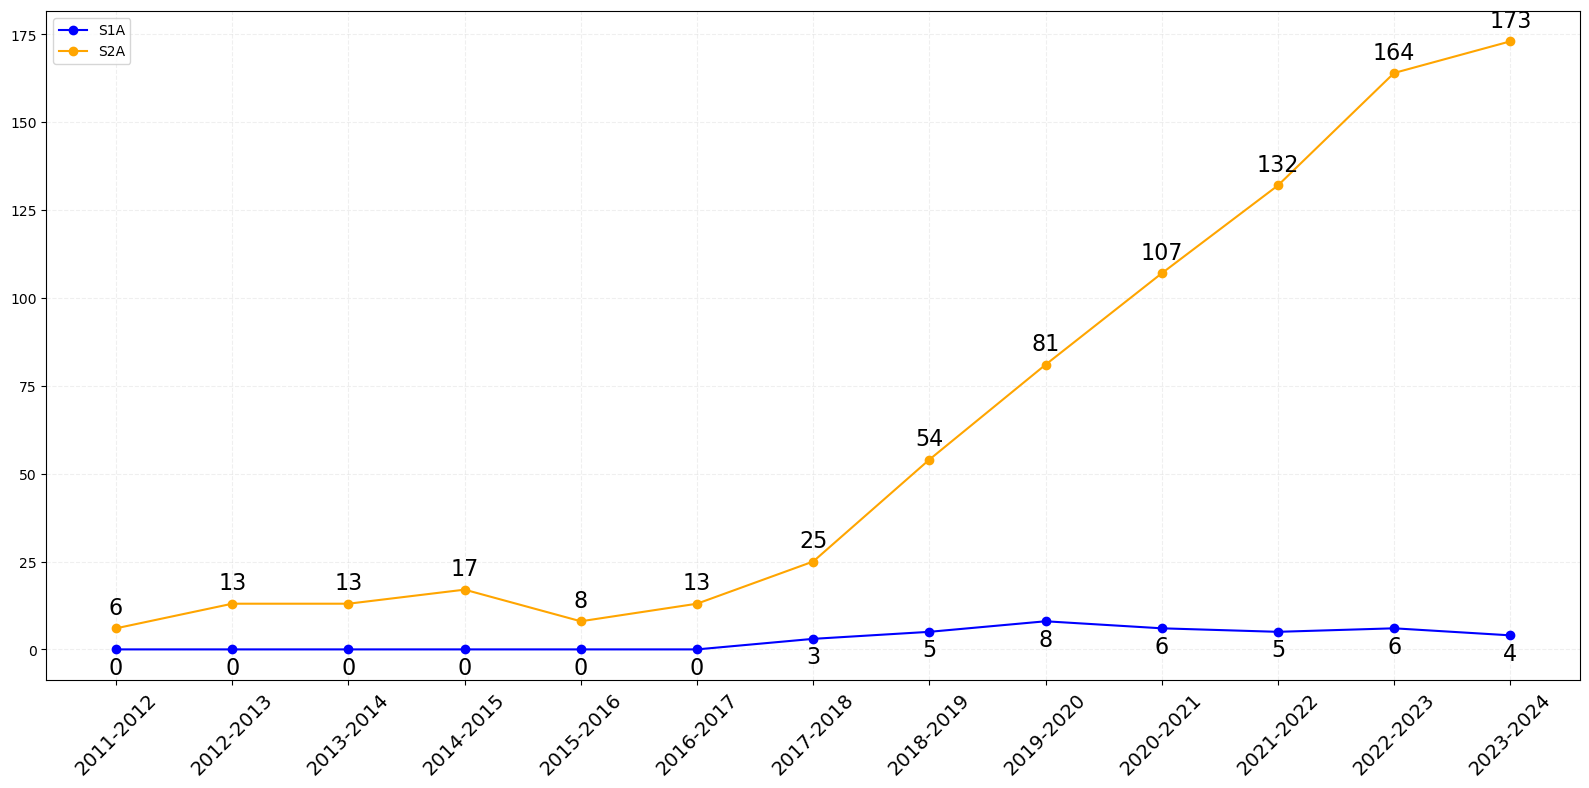
\includegraphics[width=1\textwidth]{figure/Inscrits_ucad_SA.png}
\label{fig:inscrits_ucad_sa}
\end{figure}

La figure (Figure~\ref{fig:inscrits_ucad_sa}) retrace l'évolution des inscriptions à l'UCAD pour les bacheliers des séries Sciences fondamentales (S1A) et Sciences appliquées (S2A) entre 2011-2012 et 2023-2024.

La série S1A, bien que présente, affiche un nombre d'inscrits extrêmement faible à l'UCAD tout au long de la période. Les effectifs oscillent entre 0 et 8 (atteint en 2019-2020), avec seulement 4 inscrits en 2023-2024. 
Cette quasi-absence d'inscriptions à l'université confirme le caractère très marginal de cette filière, qui déjà au niveau du baccalauréat, n'attire qu'un nombre dérisoire de candidats. 
Cela suggère que la série S1A ne débouche que sur très peu d'orientations universitaires à l'UCAD.

En revanche, la série S2A présente une dynamique d'inscriptions beaucoup plus significative. Après des débuts modestes entre 6 et 17 inscrits de 2011-2012 à 2015-2016, le nombre d'étudiants en S2A à l'UCAD connaît une croissance exponentielle. 
On passe de 25 inscrits en 2016-2017 à 107 en 2020-2021, pour atteindre un pic de 173 inscrits en 2023-2024. Cette forte augmentation des inscriptions en S2A à l'UCAD reflète une reconnaissance croissante de cette filière scientifique parmi les bacheliers arabes et franco-arabes, leur offrant des perspectives universitaires concrètes.

En somme, l'analyse des inscriptions à l'UCAD confirme les dynamiques observées au niveau du baccalauréat : la série S1A reste une filière confidentielle, tandis que la S2A gagne en importance et en attractivité pour les études supérieures, offrant ainsi une voie viable aux bacheliers issus de l'enseignement scientifique arabe et franco-arabe.

\newpage
\section{Répartition des Inscrits par Établissement et Département}

\subsection{Série STEG et G}

\subsubsection{Établissements}

\begin{figure}[ht]
\centering
\caption{Top 5 des établissements avec le plus d'inscrits (STEG, 2023-2024)}
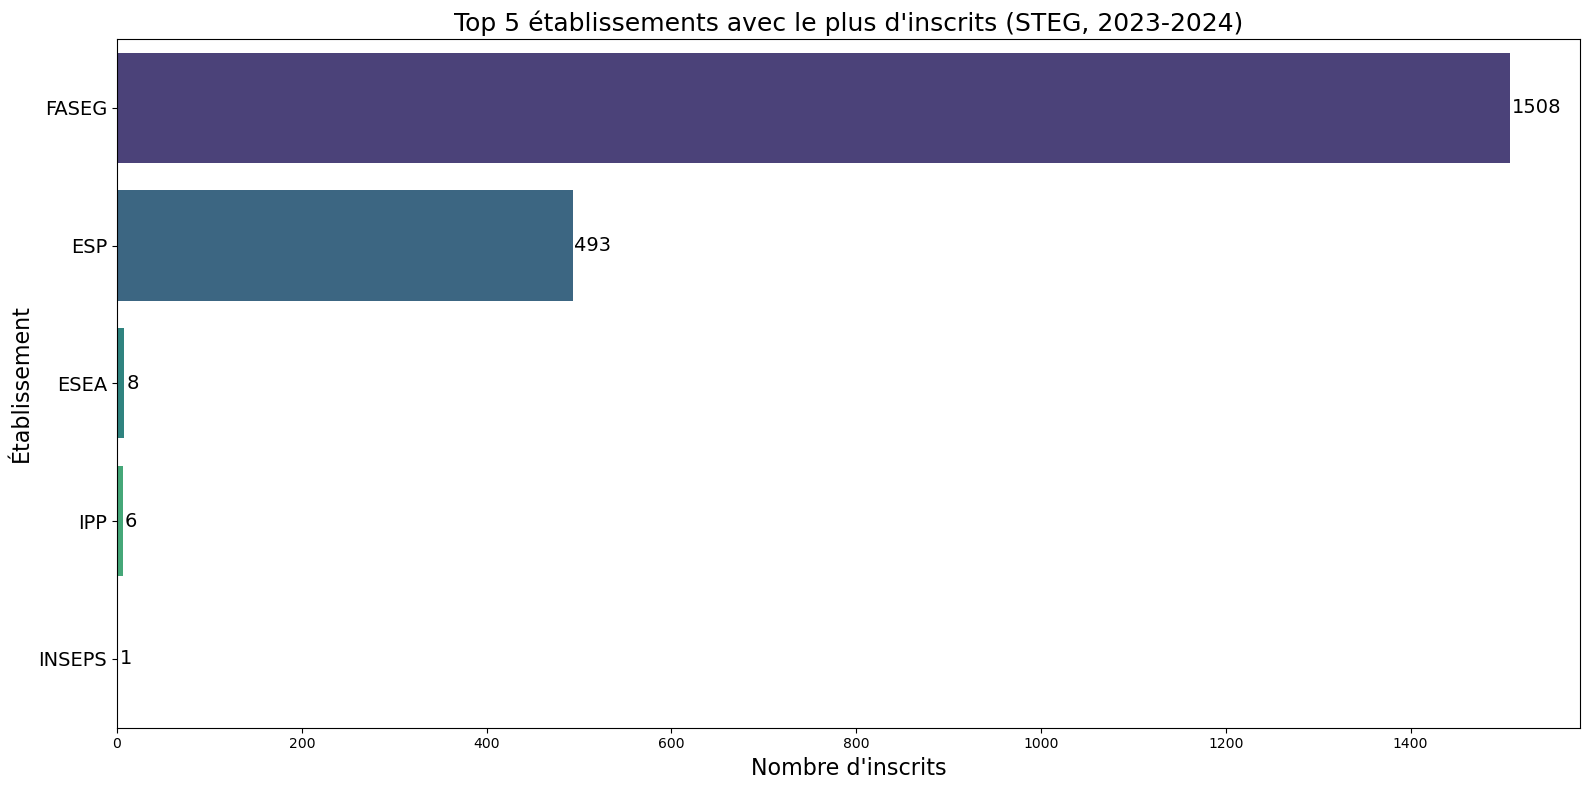
\includegraphics[width=1\textwidth]{figure/etab_STEG_2024.png}
\label{fig:etab_steg_2024}
\end{figure}

\subsubsection{Départements}

\begin{figure}[ht]
\centering
\caption{Top 5 des départements avec le plus d'inscrits (STEG, 2023-2024)}
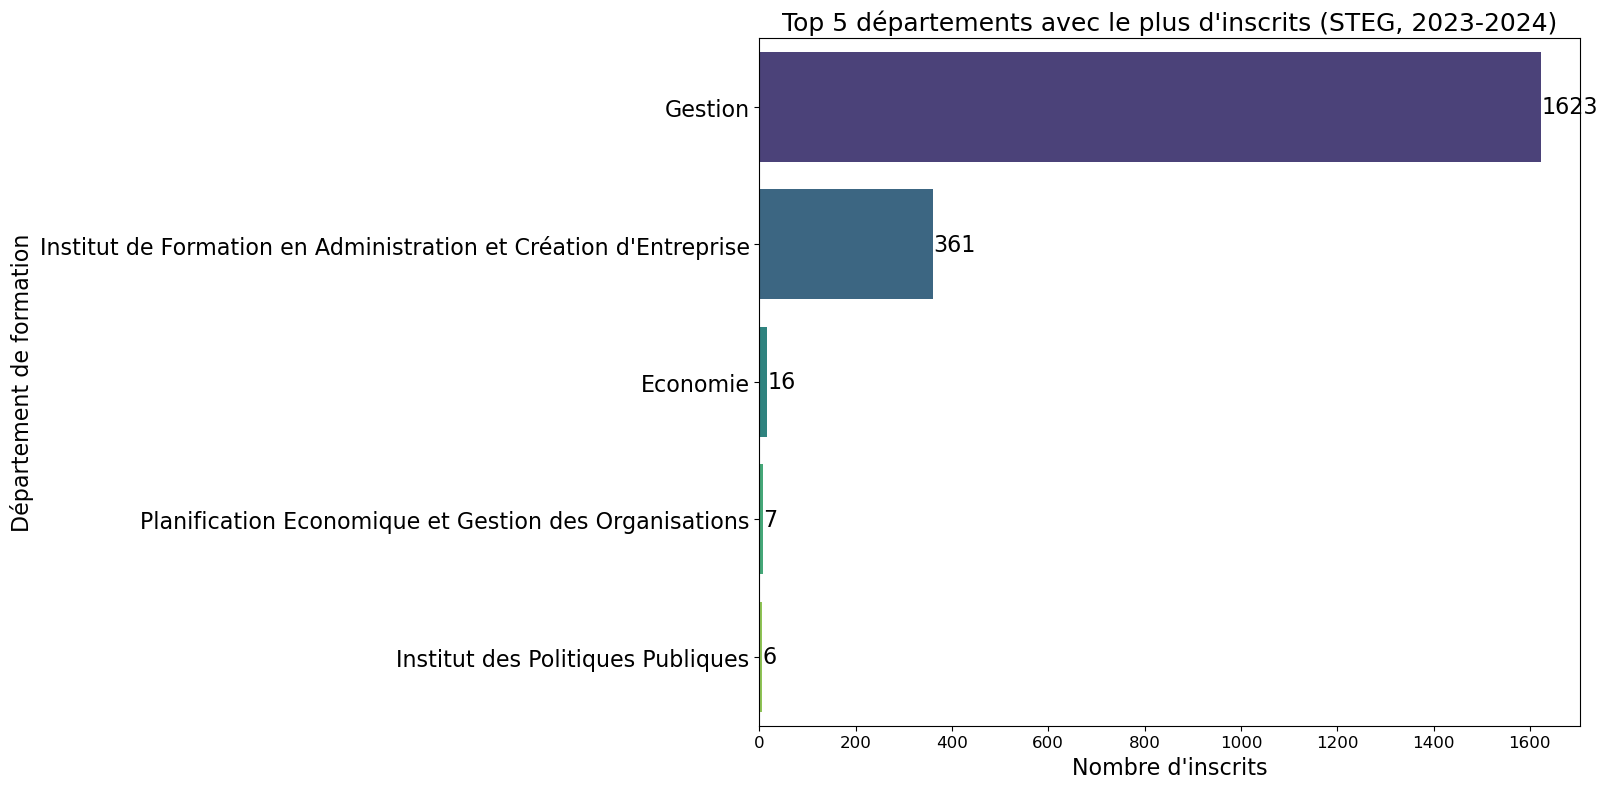
\includegraphics[width=1\textwidth]{figure/dep_STEG_2024.png}
\label{fig:dep_steg_2024}
\end{figure}

\newpage
\subsection{Série Arabes et Franco-Arabes}

\subsubsection{Série LA}

\textbf{Établissements}

\begin{figure}[ht]
\centering
\caption{Top 5 des établissements avec le plus d'inscrits (LA, 2023-2024)}
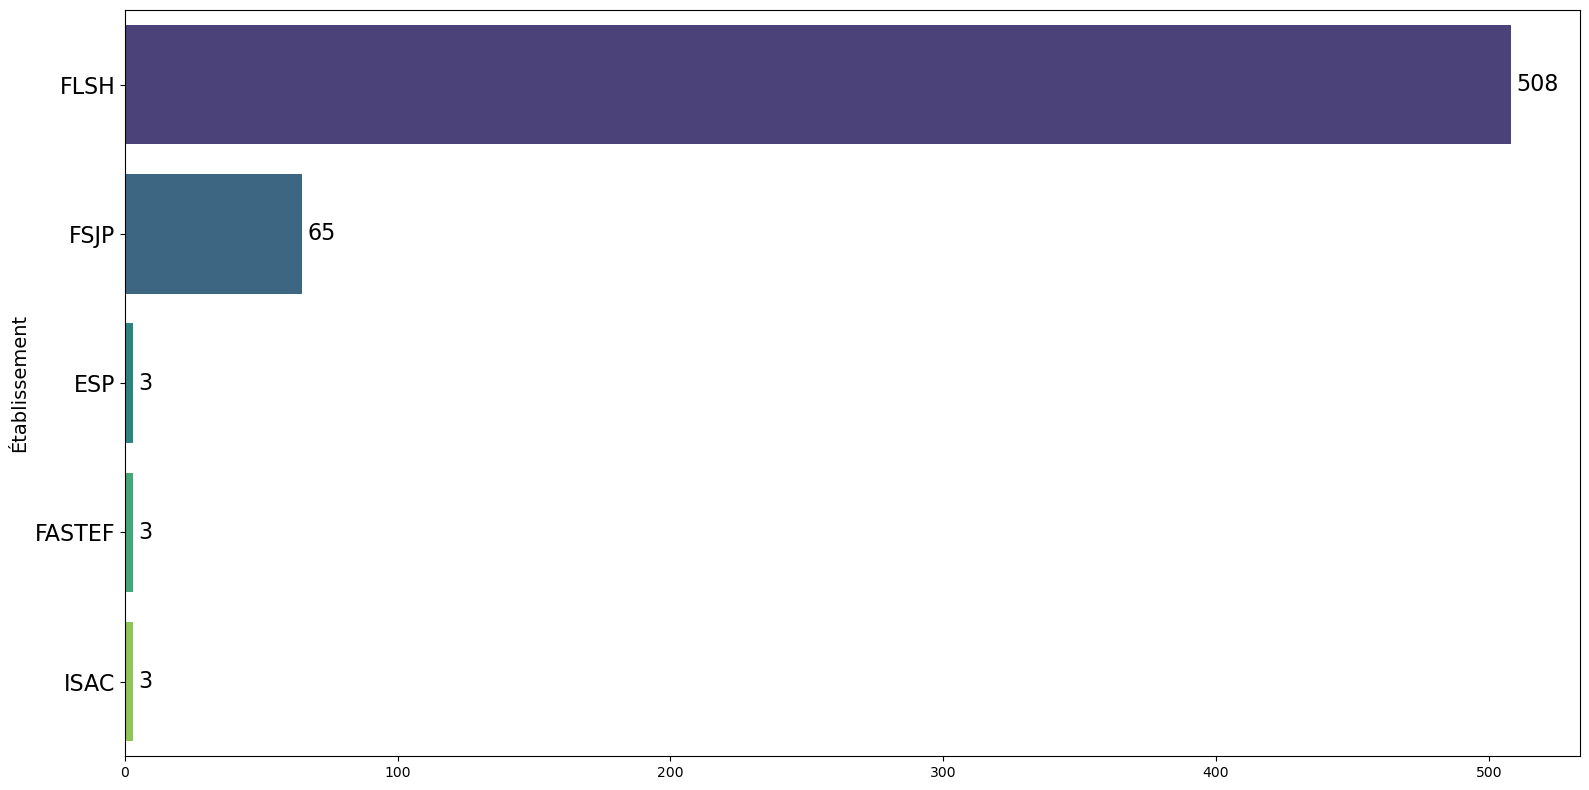
\includegraphics[width=1\textwidth]{figure/etab_LA_2024.png}
\label{fig:etab_la_2024}
\end{figure}

\textbf{Départements}

\begin{figure}[ht]
\centering
\caption{Top 5 des départements avec le plus d'inscrits (LA, 2023-2024)}
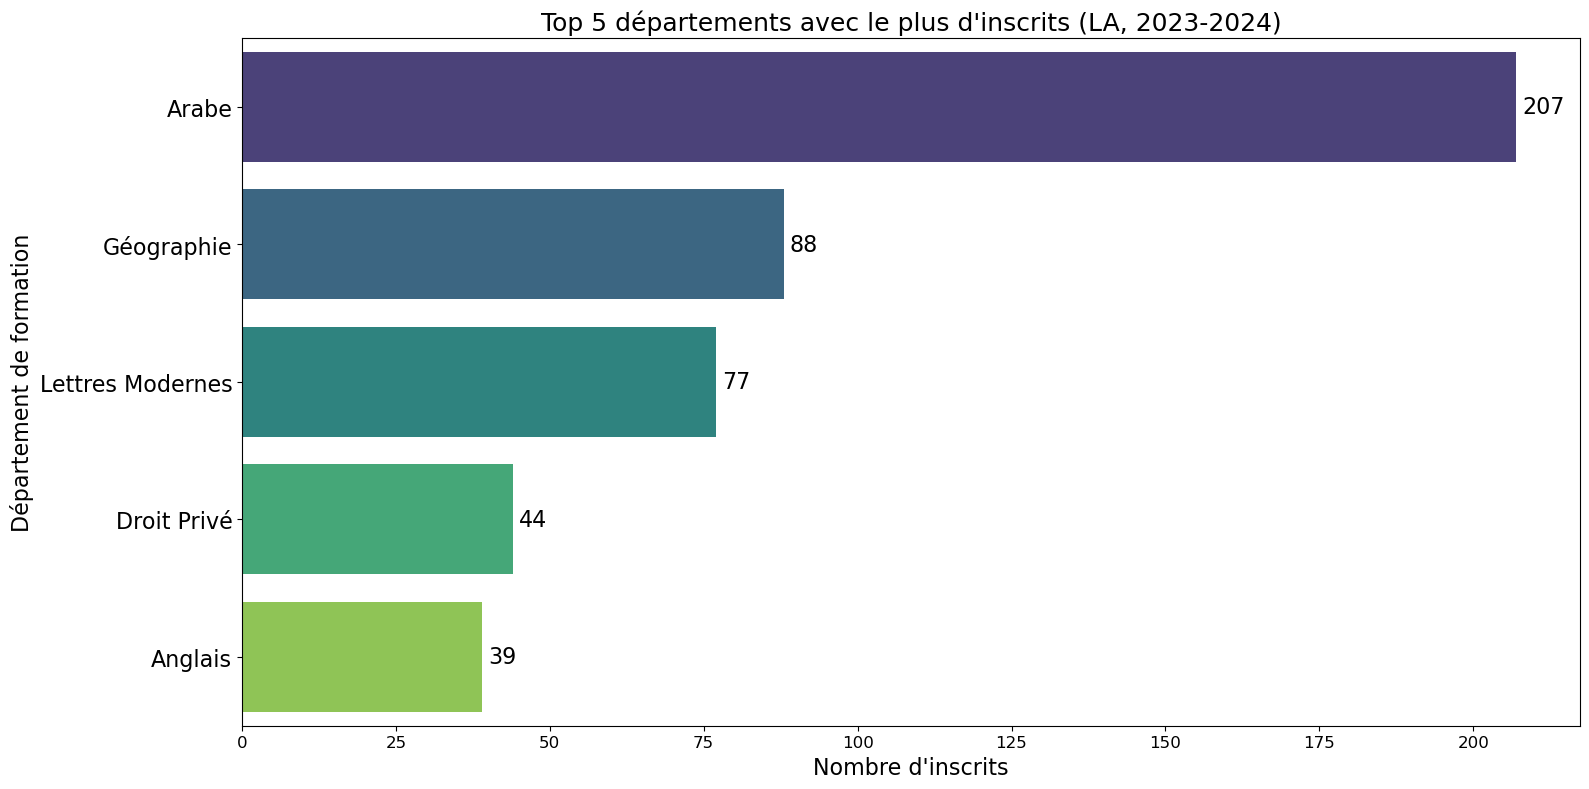
\includegraphics[width=1\textwidth]{figure/dep_LA_2024.png}
\label{fig:dep_la_2024}
\end{figure}

\newpage
\subsubsection{Série LAR}

\textbf{Établissements}

\begin{figure}[ht]
\centering
\caption{Top 5 des établissements avec le plus d'inscrits (LAR, 2023-2024)}
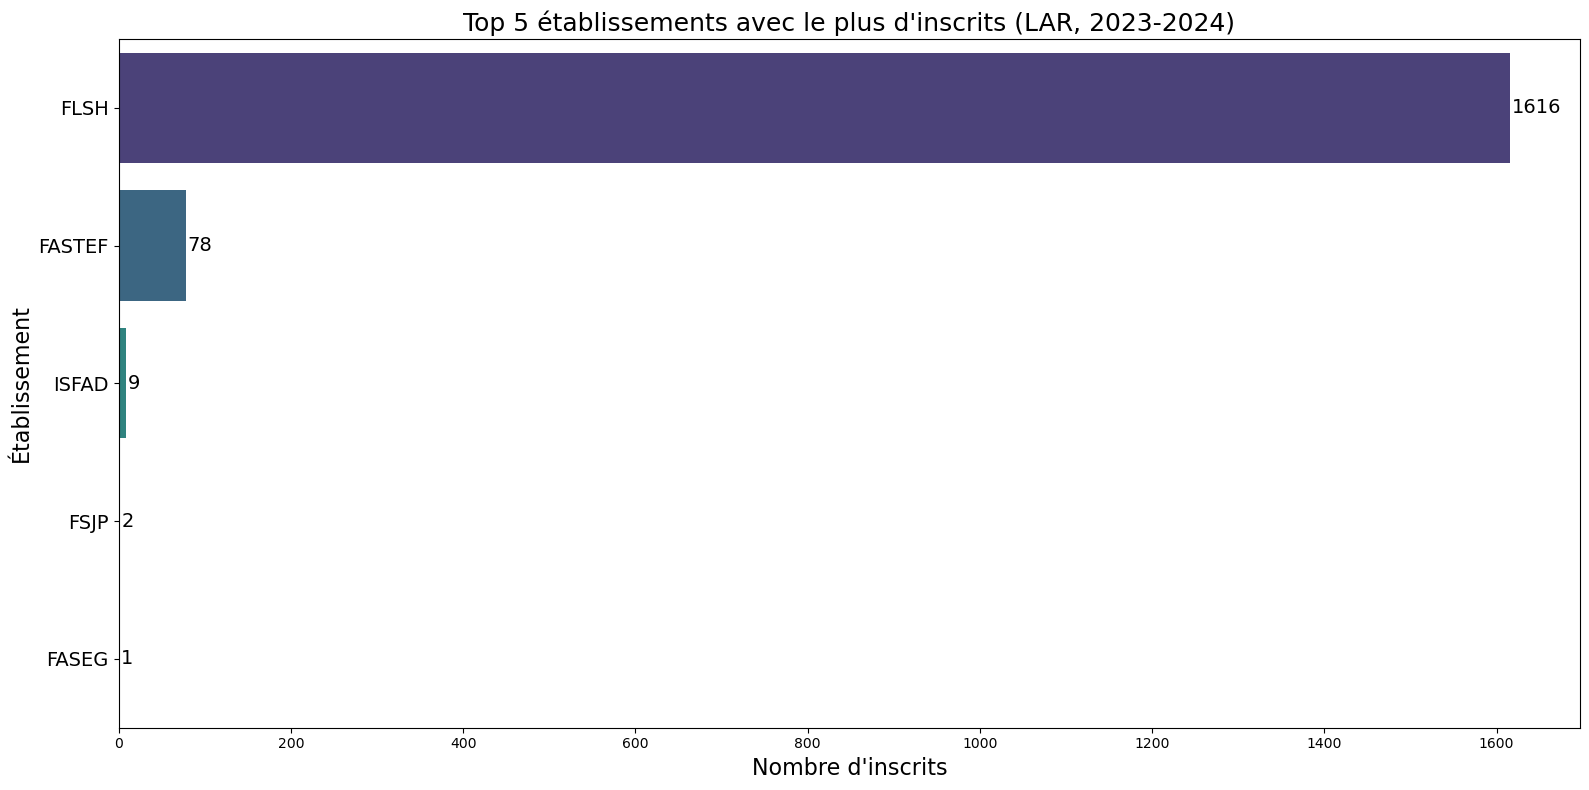
\includegraphics[width=1\textwidth]{figure/etab_LAR_2024.png}
\label{fig:etab_lar_2024}
\end{figure}

\textbf{Départements}

\begin{figure}[ht]
\centering
\caption{Top 5 des départements avec le plus d'inscrits (LAR, 2023-2024)}
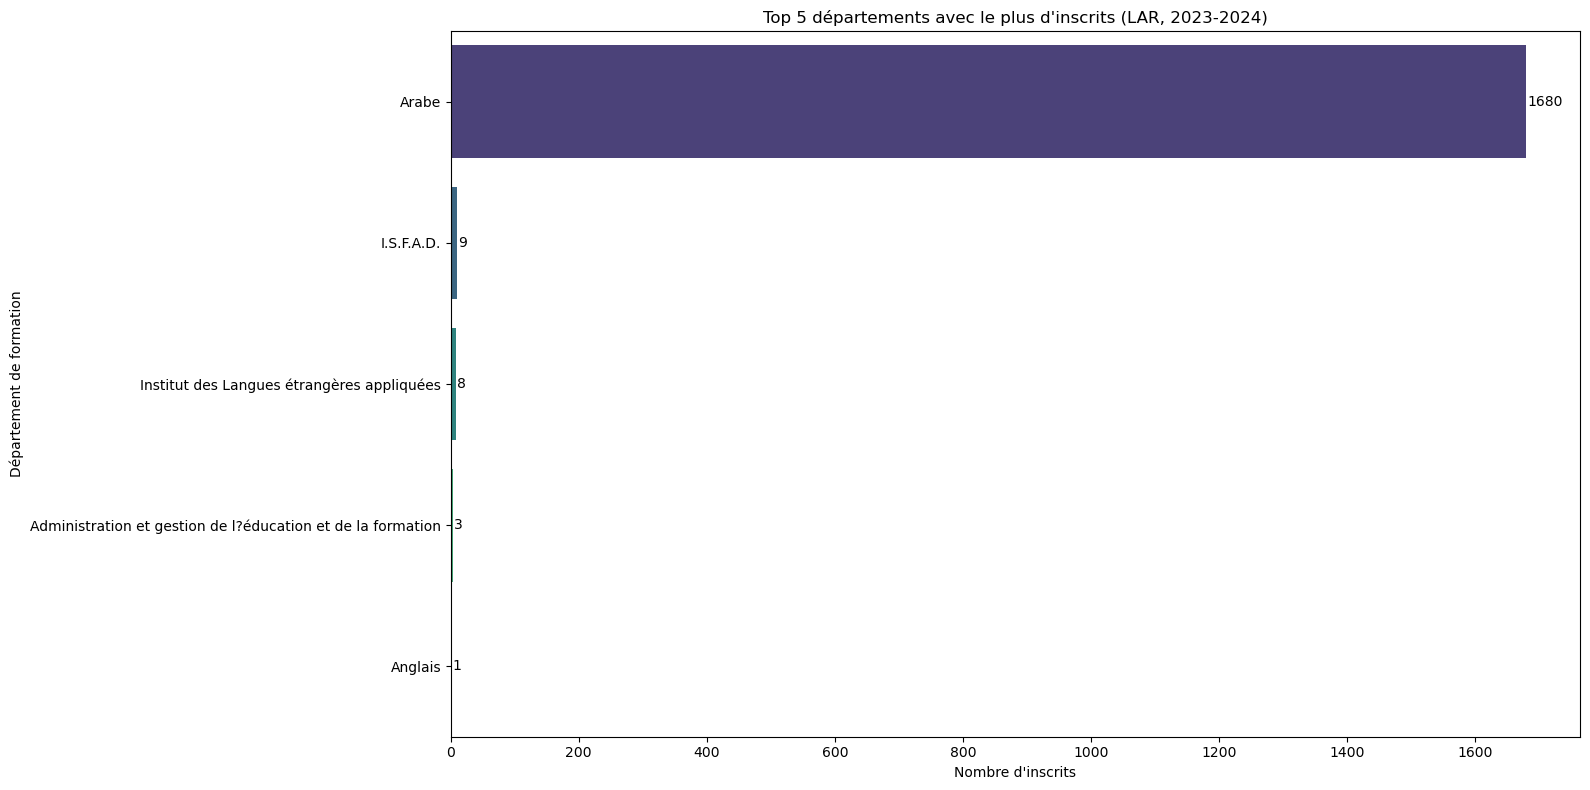
\includegraphics[width=1\textwidth]{figure/dep_LAR_2024.png}
\label{fig:dep_lar_2024}
\end{figure}

\newpage
\subsubsection{Série S2A}

\textbf{Établissements}

\begin{figure}[ht]
\centering
\caption{Top 5 des établissements avec le plus d'inscrits (S2A, 2023-2024)}
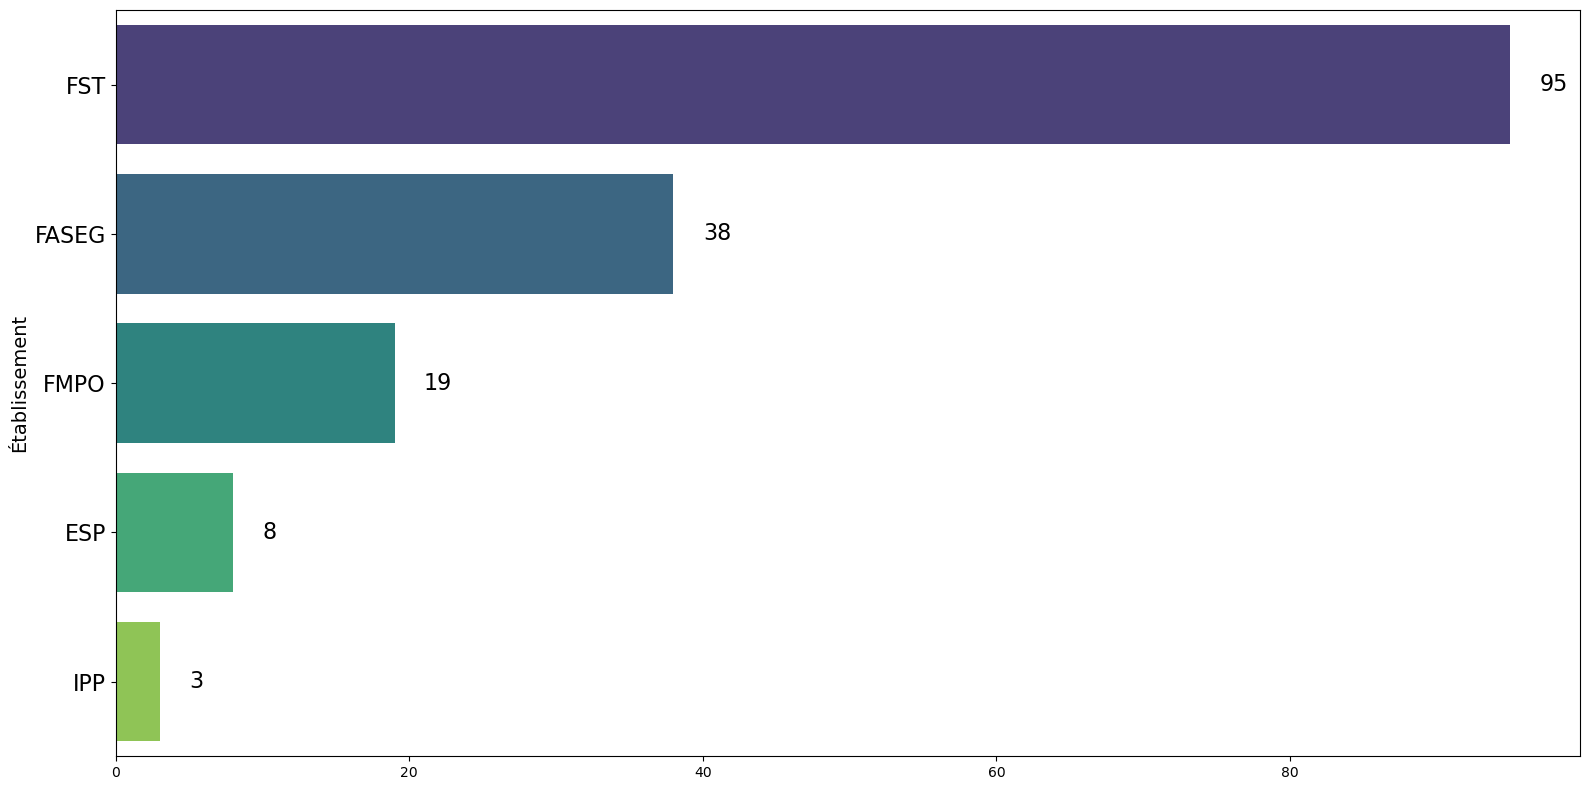
\includegraphics[width=1\textwidth]{figure/etab_S2A_2024.png}
\label{fig:etab_s2a_2024}
\end{figure}

\textbf{Départements}

\begin{figure}[ht]
\centering
\caption{Top 5 des départements avec le plus d'inscrits (S2A, 2023-2024)}
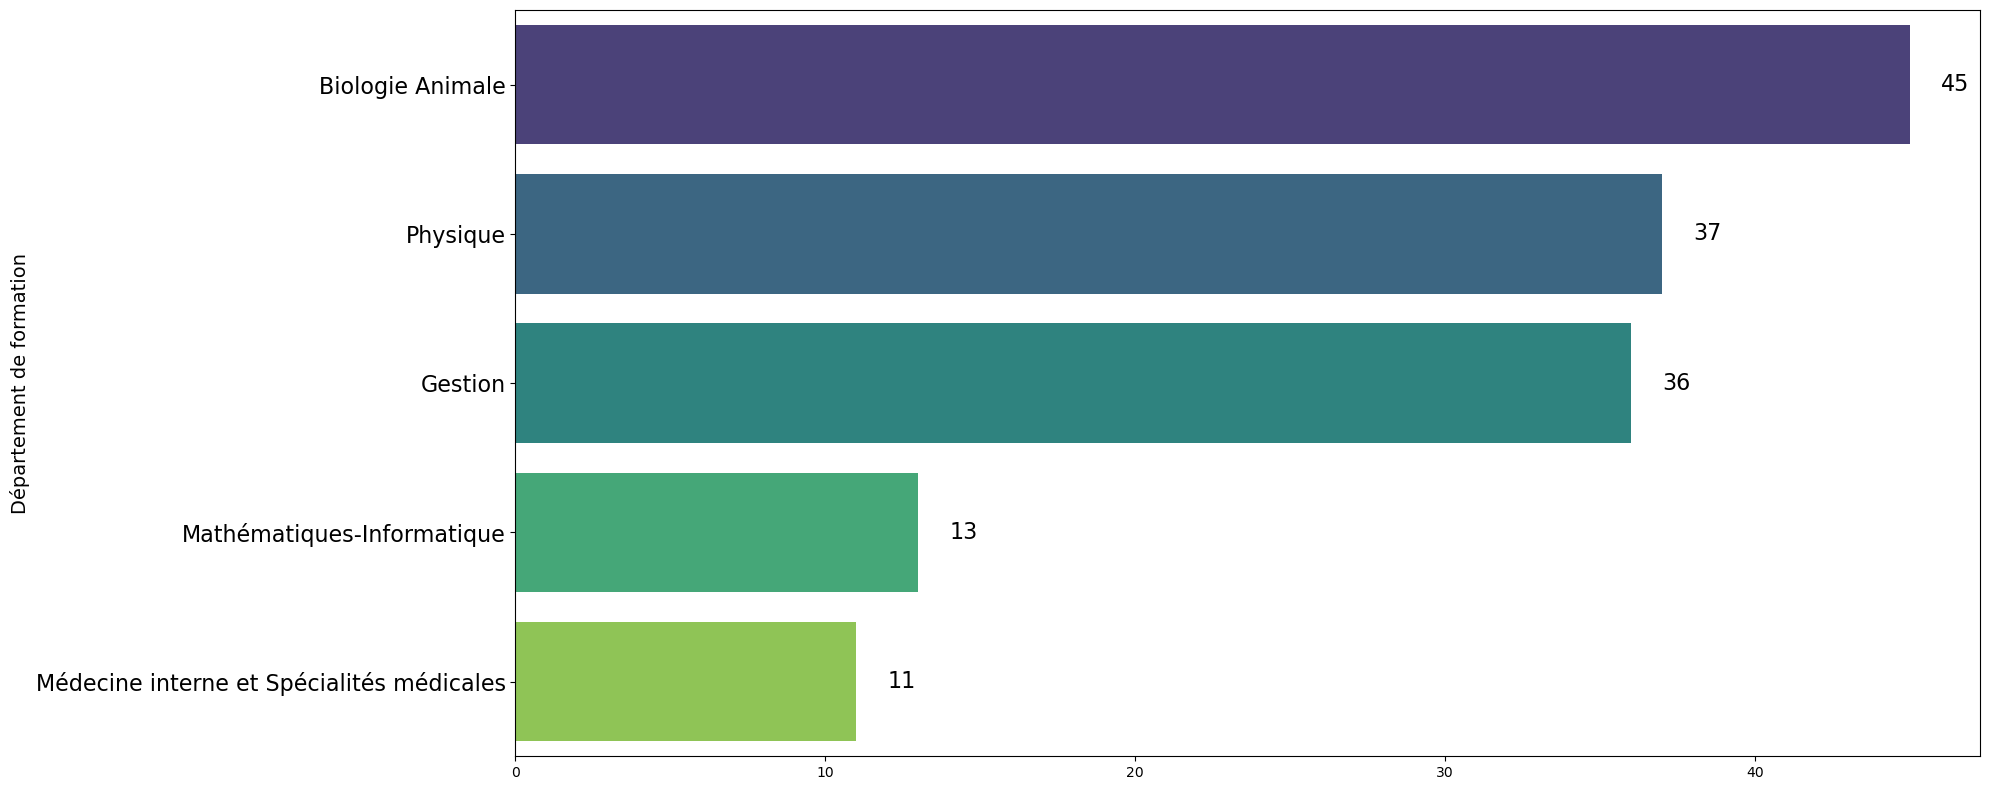
\includegraphics[width=1\textwidth]{figure/dep_S2A_2024.png}
\label{fig:dep_s2a_2024}
\end{figure}

\newpage
\subsubsection{Série S1A}

\textbf{Établissements}

\begin{figure}[ht]
\centering
\caption{Top 5 des établissements avec le plus d'inscrits (S1A, 2023-2024)}
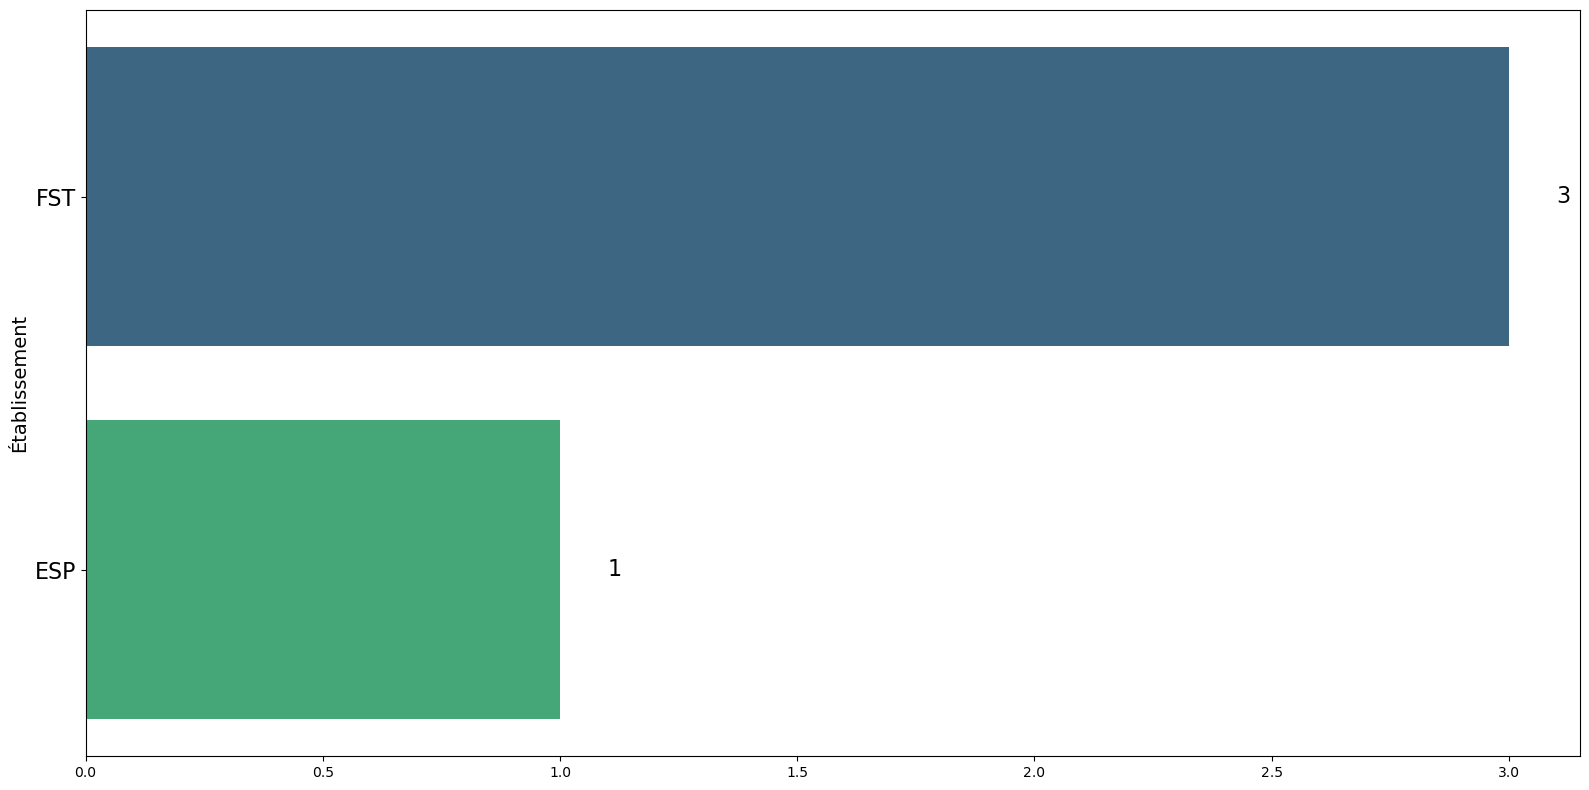
\includegraphics[width=1\textwidth]{figure/etab_S1A_2024.png}
\label{fig:etab_s1a_2024}
\end{figure}

\textbf{Départements}

\begin{figure}[ht]
\centering
\caption{Top 5 des départements avec le plus d'inscrits (S1A, 2023-2024)}
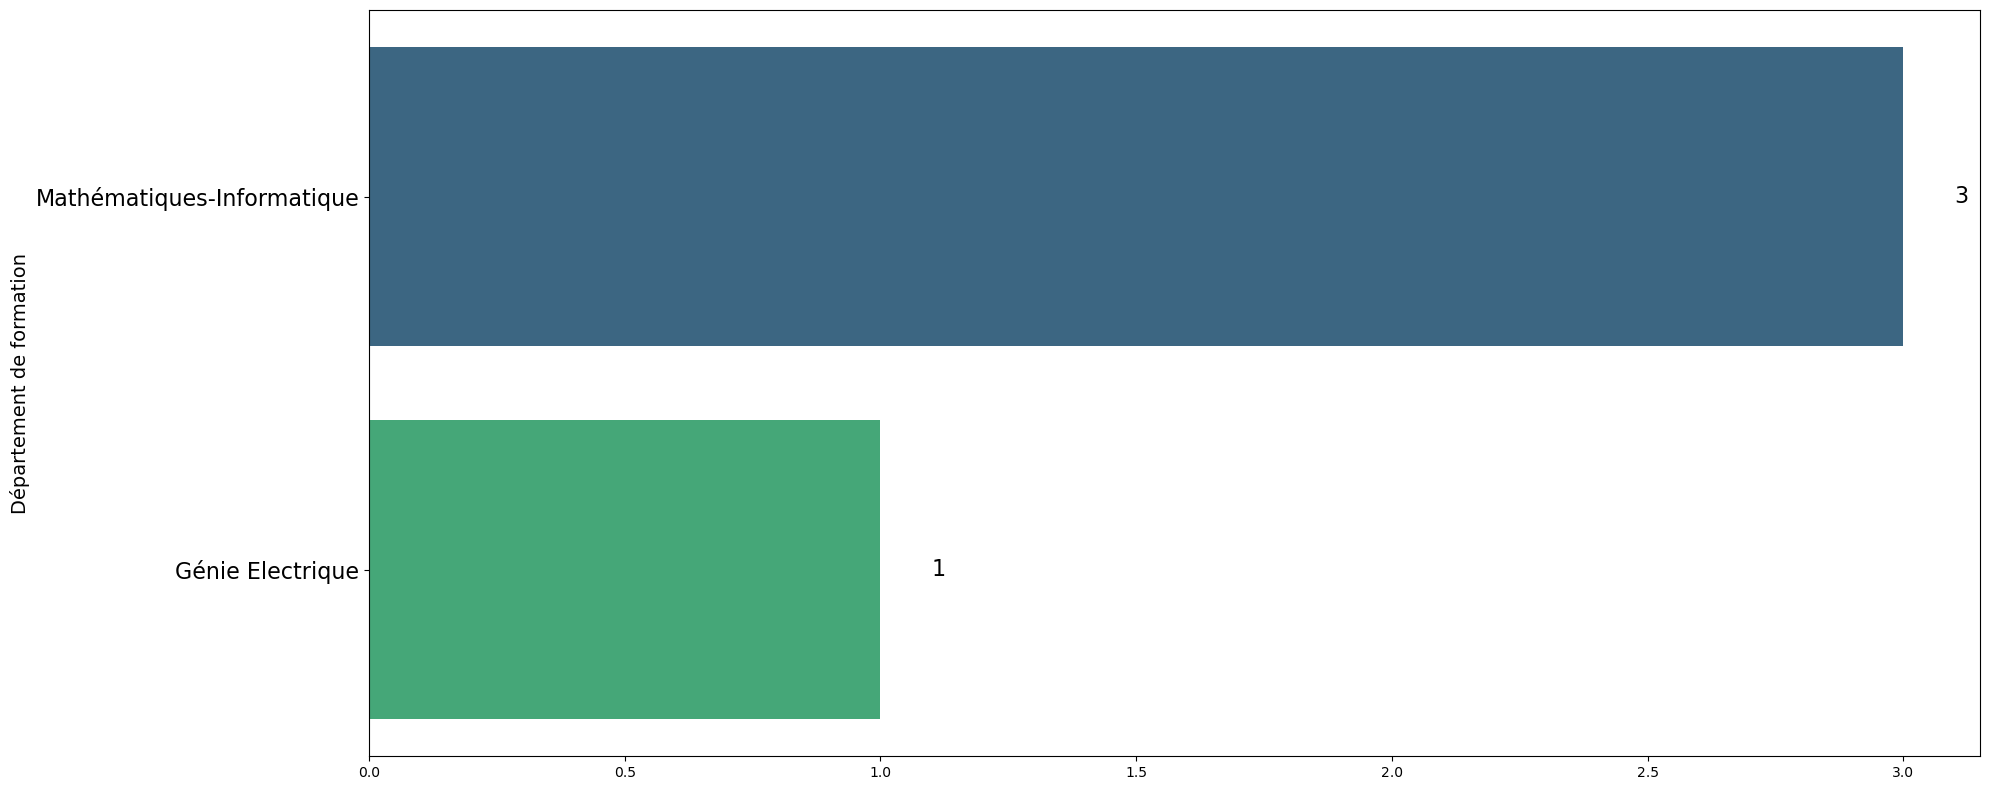
\includegraphics[width=1\textwidth]{figure/dep_S1A_2024.png}
\label{fig:dep_s1a_2024}
\end{figure}

\newpage
\section{Analyse du parcours universitaire des bacheliers (suivi des cohortes)}

\section{Conclusion}